\section{序論・問題文}
本レポートは「2D match move/augmented reality」を選択した。

近年、スポーツに使用されるスタジアムのバックネット広告に、
バーチャル広告が採用されているケースがある。
例えば2018年のボルシア・ドルトムントではビッチわきの広告版にこの技術を採用し、
ヨーロッパやアメリカ、アジアそれぞれの試合中継で異なる広告を表示することで広告板を増やすことなく広告スペースを拡大することに成功している\cite{bvb}。

本レポートではこのバーチャル広告のベースとなる技術を実装する。
具体的には画像のワーピング、特徴量抽出及びマッチング、ホモグラフィ行列の算出を組み合わせて、対象画像の一部を差し替える。

問題の全体像を以下の図に示す。まず、図\ref{fig:question}(a)の部分画像ABCD(テンプレート画像)とマッチする部分画像EFGH(適用画像)を図中(c)から探索する。その後図中(b)の差し替え先画像から差し替え画像へのホモグラフィ行列を計算し、ワーピング処理によって差し替えを行う。

\begin{figure}[h]
    \centering
    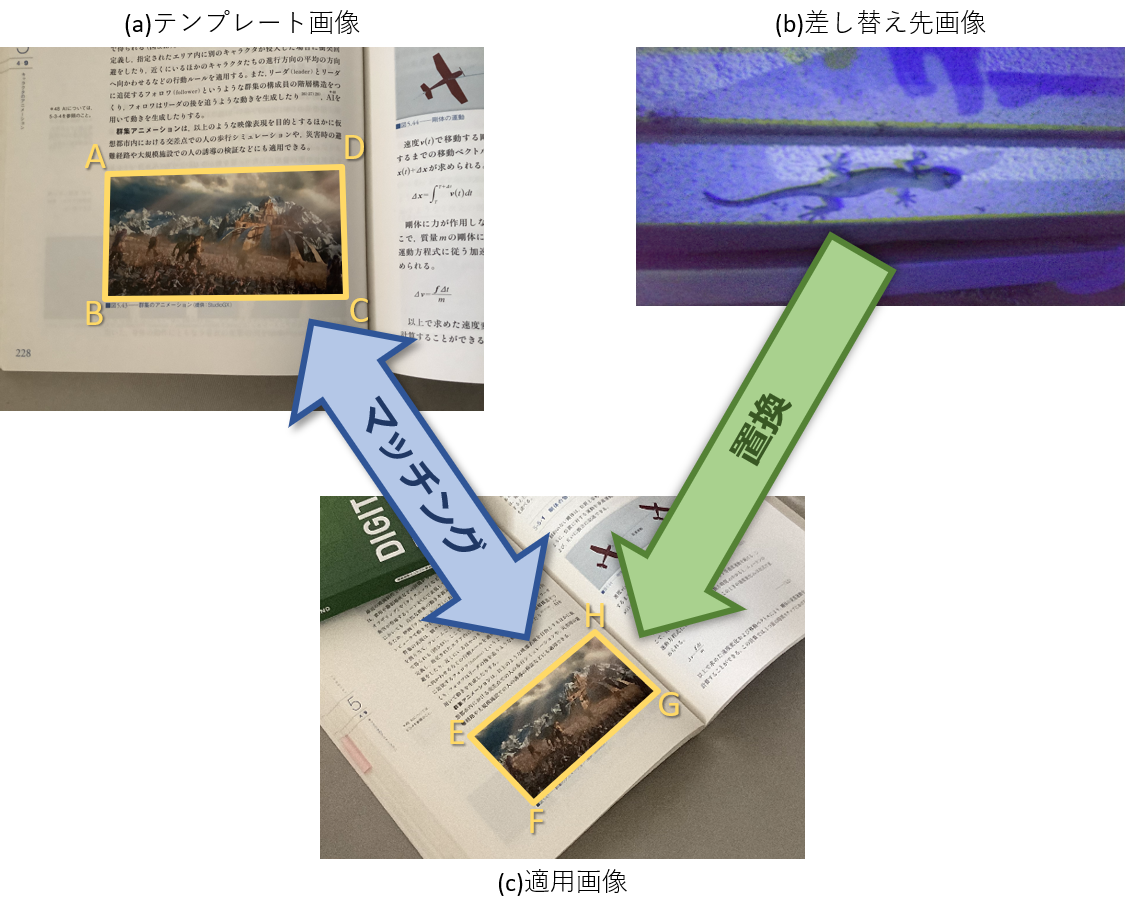
\includegraphics[width=1\linewidth]{fig/question.png}
    \caption{問題の全体像}
    \label{fig:question}
\end{figure}

以降の章の構成は次の通りである。
\ref{sec:impl}章では本アプリケーションで使用するアルゴリズムおよび実装を示す。
\ref{sec:eval}章では実装したアプリケーションの検出精度や実行時間などを評価する。
最後に\ref{sec:conc}で本レポートの結論を述べる。